\UseRawInputEncoding
\documentclass[12pt]{article}
\usepackage[utf8]{inputenc}

\usepackage[T1]{fontenc}
\usepackage[spanish]{babel}
\usepackage{listings}
\usepackage{xcolor}
\usepackage{graphicx}
\usepackage{geometry}
\geometry{margin=2.5cm}

\title{Documentación de la Interfaz de Usuario - Juego Mancala}
\author{
  Juan Andrés Rodríguez Rubio \\
  Carlos Enrique Caicedo Guerrero \\
  Alejandro Caicedo Caicedo
}
\date{}

% Configuración para listings (código)
\lstset{
  basicstyle=\ttfamily\small,
  backgroundcolor=\color{gray!10},
  frame=single,
  framerule=0pt,
  language=Python,
  showstringspaces=false
}

\lstset{literate= % permite utilizar tildes y otros símbolos dentro del código
	{á}{{\'a}}1 {é}{{\'e}}1 {í}{{\'i}}1 {ó}{{\'o}}1 {ú}{{\'u}}1
	{Á}{{\'A}}1 {É}{{\'E}}1 {Í}{{\'I}}1 {Ó}{{\'O}}1 {Ú}{{\'U}}1
	{à}{{\`a}}1 {è}{{\`e}}1 {ì}{{\`i}}1 {ò}{{\`o}}1 {ù}{{\`u}}1
	{À}{{\`A}}1 {È}{{\'E}}1 {Ì}{{\`I}}1 {Ò}{{\`O}}1 {Ù}{{\`U}}1
	{ä}{{\"a}}1 {ë}{{\"e}}1 {ï}{{\"i}}1 {ö}{{\"o}}1 {ü}{{\"u}}1
	{Ä}{{\"A}}1 {Ë}{{\"E}}1 {Ï}{{\"I}}1 {Ö}{{\"O}}1 {Ü}{{\"U}}1
	{â}{{\^a}}1 {ê}{{\^e}}1 {î}{{\^i}}1 {ô}{{\^o}}1 {û}{{\^u}}1
	{Â}{{\^A}}1 {Ê}{{\^E}}1 {Î}{{\^I}}1 {Ô}{{\^O}}1 {Û}{{\^U}}1
	{œ}{{\oe}}1 {Œ}{{\OE}}1 {æ}{{\ae}}1 {Æ}{{\AE}}1 {ß}{{\ss}}1
	{ű}{{\H{u}}}1 {Ű}{{\H{U}}}1 {ő}{{\H{o}}}1 {Ő}{{\H{O}}}1
	{ç}{{\c c}}1 {Ç}{{\c C}}1 {ø}{{\o}}1 {å}{{\r a}}1 {Å}{{\r A}}1
	{€}{{\EUR}}1 {£}{{\pounds}}1 {~}{{$\sim$}}1
}

\begin{document}

\maketitle

\section{Descripción General}

Este documento presenta una descripción de la interfaz de usuario del juego clásico \textbf{Mancala}, implementado en Python para ser ejecutado desde la consola. El juego permite la participación de dos jugadores que se turnan para distribuir piedras y aplicar las reglas tradicionales del Mancala.

\section{Reglas del Juego}

\begin{itemize}
    \item Cada jugador dispone de 6 pozos, cada uno con 4 piedras al inicio de la partida.
    \item Cada jugador posee una \textbf{Mancala} (depósito) donde acumula las piedras capturadas.
    \item Durante su turno, el jugador selecciona uno de sus pozos y distribuye sus piedras en sentido horario.
    \item Si la última piedra cae en su propia Mancala, el jugador obtiene un turno adicional.
    \item Si la última piedra cae en un pozo vacío del propio lado y el pozo opuesto contiene piedras, se realiza una \textbf{captura}.
    \item La partida finaliza cuando un jugador ya no tiene piedras en sus pozos.
    \item Gana el jugador que acumule la mayor cantidad de piedras en su Mancala.
\end{itemize}
\section{Descripcion del codigo}
\subsection{Diseño de la clase \textbf{Mancala}}
Se diseñó una clase que está conformada por dos atributos:
\begin{itemize}
    \item \texttt{board}: Lista que representa el tablero con 14 posiciones:
    \begin{itemize}
        \item Posiciones 0-5: Pozos del jugador 1
        \item Posición 6: Mancala del jugador 1
        \item Posiciones 7-12: Pozos del jugador 2
        \item Posición 13: Mancala del jugador 2
    \end{itemize}
    \item \texttt{player\_turn}: Indica qué jugador tiene el turno (1 o 2)
\end{itemize}

\subsubsection{Constructor \_\_init\_\_}
Inicializa el tablero de juego y establece el turno del jugador 1.
\begin{lstlisting}[language=Python]
def __init__(self):
    # Inicializar el tablero: 6 pozos para cada jugador y 1 mancala
    self.board = [4] * 6 + [0] + [4] * 6 + [0]
    self.player_turn = 1  # Jugador 1 comienza
\end{lstlisting}
\subsubsection{Método print\_board}
Imprime por consola el estado actual del tablero.
\begin{lstlisting}[language=Python]
def print_board(self):
    print("\nTablero:")
    print("Jugador 2 (Mancala: {})".format(self.board[13]))
    print ("Posicion fichas: 12  11  10  9  8  7")
    print("Pozo jugador 2: ", self.board[12:6:-1])
    print("Pozo jugador 1 ", self.board[0:6])
    print ("Posicion fichas: 0  1  2  3  4  5")
    print("Jugador 1 (Mancala: {})".format(self.board[6]))
    print("Turno del Jugador", self.player_turn)
\end{lstlisting}

\subsubsection{Método make\_move}
Realiza un movimiento en el juego según el pozo seleccionado. En primer lugar, se valida si el movimiento está de acuerdo con las reglas establecidas. En caso contrario, se muestra un mensaje de error al usuario. Si el movimiento es válido, se colocan las piedras en los lugares adecuados y se hacen las verificaciones necesarias de acuerdo con las reglas del juego. Después de revisar si se aplican saltos de mancala o capturas de piedras, se pasa el turno al siguiente jugador.

\begin{lstlisting}[language=Python]
def make_move(self, pit):
    # Validación del movimiento
    if self.player_turn == 1:
        if pit < 0 or pit > 5 or self.board[pit] == 0:
            print("Movimiento inválido. Intenta de nuevo.")
            return False
    else:
        if pit < 7 or pit > 12 or self.board[pit] == 0:
            print("Movimiento inválido. Intenta de nuevo.")
            return False

    # Distribución de las piedras
    stones = self.board[pit]
    self.board[pit] = 0
    current_pit = pit

    while stones > 0:
        current_pit = (current_pit + 1) % 14
        if (self.player_turn == 1 and current_pit == 13) or 
                (self.player_turn == 2 and current_pit == 6):
            continue  # Saltar el mancala del oponente
        self.board[current_pit] += 1
        stones -= 1

    # Captura de piedras
    if self.board[current_pit] == 1 and 
            ((self.player_turn == 1 and 0 <= current_pit <= 5) or 
            (self.player_turn == 2 and 7 <= current_pit <= 12)):
        opposite_pit = 12 - current_pit
        if self.board[opposite_pit] > 0:
            self.board[6 if self.player_turn == 1 else 13] += 
                self.board[opposite_pit] + 1
            self.board[current_pit] = 0
            self.board[opposite_pit] = 0

    # Cambio de turno
    if (self.player_turn == 1 and current_pit != 6) or 
            (self.player_turn == 2 and current_pit != 13):
        self.player_turn = 3 - self.player_turn

    return True
\end{lstlisting}

\subsubsection{Método check\_game\_over}
Verifica si el juego ha terminado (cuando todos los pozos de un jugador están vacíos).

\begin{lstlisting}[language=Python]
def check_game_over(self):
    if all(stones == 0 for stones in self.board[0:6]) or 
            all(stones == 0 for stones in self.board[7:13]):
        self.board[6] += sum(self.board[0:6])
        self.board[13] += sum(self.board[7:13])
        for i in range(14):
            if i != 6 and i != 13:
                self.board[i] = 0
        return True
    return False
\end{lstlisting}

\subsubsection{Método get\_winner}
Determina el ganador del juego comparando las piedras en los mancalas.

\begin{lstlisting}[language=Python]
def get_winner(self):
    if self.board[6] > self.board[13]:
        return "Jugador 1"
    elif self.board[6] < self.board[13]:
        return "Jugador 2"
    else:
        return "Empate"
\end{lstlisting}

\subsection{Función principal}
La función \texttt{main()} controla el flujo del juego.

\begin{lstlisting}[language=Python]
def main():
    game = Mancala()
    while True:
        game.print_board()
        if game.player_turn == 1:
            pit = int(input("Jugador 1, elige un pozo (0-5): "))
        else:
            pit = int(input("Jugador 2, elige un pozo (7-12): "))

        if not game.make_move(pit):
            continue

        if game.check_game_over():
            game.print_board()
            print("¡Juego terminado!")
            print("El ganador es:", game.get_winner())
            break
\end{lstlisting}


\section{Interfaz por Consola}

A continuación se presenta un ejemplo de salida en consola:

\begin{lstlisting}
Tablero:
Jugador 2 (Mancala: 0)
Posicion fichas: 12  11  10  9  8  7
Pozo jugador 2:  [4, 4, 4, 4, 4, 4]
Pozo jugador 1  [4, 4, 4, 4, 4, 4]
Posicion fichas: 0  1  2  3  4  5
Jugador 1 (Mancala: 0)
Turno del Jugador 1
Jugador 1, elige un pozo (0-5):
\end{lstlisting}

\textbf{Descripción de la salida:}

\begin{itemize}
    \item \texttt{Jugador 2 (Mancala: 0)}: Muestra la cantidad de piedras acumuladas por el Jugador 2.
    \item \texttt{Pozo jugador 2}: Representa el estado de los pozos del Jugador 2 (posiciones de la 12 a la 7).
    \item \texttt{Pozo jugador 1}: Representa el estado de los pozos del Jugador 1 (posiciones de la 0 a la 5).
    \item \texttt{Jugador 1 (Mancala: 0)}: Muestra la cantidad de piedras acumuladas por el Jugador 1.
    \item \texttt{Turno del Jugador 1}: Indica a quién corresponde realizar el siguiente movimiento.
    \item \texttt{Jugador 1, elige un pozo (0-5)}: Solicita al jugador que seleccione el pozo desde el cual desea mover.
\end{itemize}

\begin{figure}[h!]
    \centering
    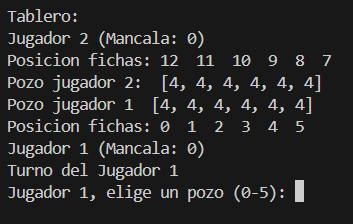
\includegraphics[width=0.9\textwidth]{Tablero.png}
    \caption{Vista del tablero del juego en consola}
    \label{fig:tablero}
\end{figure}

\section{Errores Comunes}

\begin{itemize}
    \item Seleccionar un pozo fuera del rango permitido.
    \item Seleccionar un pozo que no contiene piedras.
\end{itemize}

En cualquiera de estos casos, el sistema mostrará el siguiente mensaje:

\begin{lstlisting}
Movimiento invalido. Intenta de nuevo.
\end{lstlisting}

\begin{figure}[h!]
    \centering
    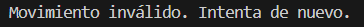
\includegraphics[width=0.6\textwidth]{Error.png}
    \caption{Ejemplo de mensaje por movimiento inválido}
    \label{fig:error}
\end{figure}

\section*{Ejecución del Programa}

Para ejecutar el juego, se debe contar con \textbf{Python 3} instalado en el sistema. Una vez ubicado en el directorio del archivo \texttt{mancala.py}, se debe ingresar el siguiente comando en la terminal o consola:

\begin{verbatim}
python mancala.py
\end{verbatim}

\begin{figure}[h!]
    \centering
    
\includegraphics[width=0.65\textwidth]{Ejecutar.png}
    \caption{Ejemplo del comando para ejecutar el juego}
    \label{fig:ejecutar}
\end{figure}

\section{Recomendaciones Generales}

\begin{itemize}
    \item Verificar que el archivo se encuentre correctamente nombrado como \texttt{mancala.py}.
    \item No cerrar la consola mientras la partida esté en curso.
    \item Puede reiniciar el juego simplemente ejecutando el archivo nuevamente.
\end{itemize}

\end{document}
